\section{项目的主要内容和技术路线}

\subsection{主要研究内容}

本研究的方向是通过模糊测试进行并发漏洞的挖掘,主要对以下几方面进行研究:

\begin{enumerate}
\item 对模糊测试的相关工具进行评估,并对特定的针对并发访问漏洞的工具进行研究和评估。
\item 寻找更有效的进行线程交错空间探索的方法。
\item 对于模糊测试的反馈,寻找更加合适的指标以反应当前对线程交错空间探索的程度。
\item 开发高效的算法,能够在更加系统化地探索线程交错空间的同时保证探索的效率,在稀疏的线程交错空间中寻找到有效的测试用例。
\item 探索复现机制,能够在模糊测试系统发现特定的漏洞后给出详细准确的报告,并复现出并发访问漏洞的情况。
\item 结合其他方式(如静态分析,动态分析)的手段,改进模糊测试的效率。
\item 如果可以在用户程序以及内核上实现良好的检测效果,则应进一步探索在其他系统如物联网系统上的效果,并结合物联网系统的特点尝试进行进一步的发展。
\end{enumerate}

\subsection{技术路线}

主要采用三步,分别是静态分析,单线程模糊测试,多线程模糊测试。

\begin{enumerate}
\item 静态分析
\begin{enumerate}
\item 利用 point-to-analysis 得到所有的冲突指令对。
\item 将所有的冲突指令对作为一个集合,并筛选其中不符合要求的指令对。
\end{enumerate}

\item 单线程模糊测试
\begin{enumerate}
\item 对目标程序进行静态分析,得到线程的列表。
\item 开启单线程下的模糊测试,通过单线程下的模糊测试对线程下的代码执行路径进行探索,并记录下探索的过程中发现的访存指令。
\item 在获取到了所有线程的每一个访存指令之后,建立一个表,表中每一条访存指令对应于多个输入。
\end{enumerate}

\item 多线程模糊测试
\begin{enumerate}
\item 对多个指令对,针对其中的每个指令对,在指令之前插入断点,使其能够在指令位置按照顺序执行。
\item 在执行的过程中收集交错覆盖反馈信息,并基于此对输入进行变异,继续进行测试。
\end{enumerate}

\end{enumerate}

\subsection{可行性分析}

在利用模糊测试进行并发访问检测的领域中,目前已经有一些比较好的尝试和成果,如\autoref{fig:fig4}所示.

\begin{figure}[ht]
    \centering
    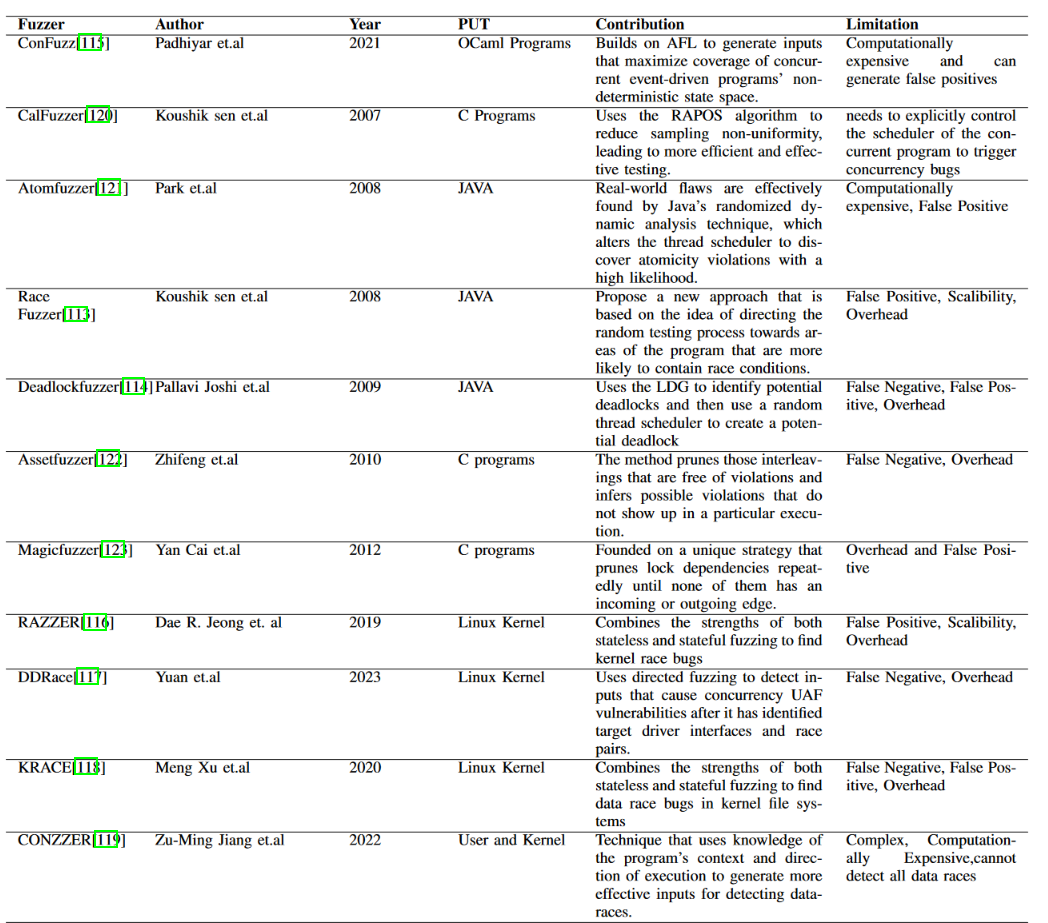
\includegraphics[width=0.8\linewidth]{fig4}
    \caption{\label{fig:fig4}一些利用模糊测试挖掘并发访问漏洞的工作}
\end{figure}

其中最近几年的工作如RAZZER\cite{jeong2019razzer},KRACE\cite{xu2020krace},CONZZER\cite{jiang2022context},DDRace\cite{yuan2023ddrace}都在利用模糊测试发掘并发访问漏洞上做出了一定的贡献,并且都能在特定的场景下得到比较好的效果,这证明使用模糊测试来进行并发访问漏洞挖掘是可行的。同时上面的几份工作测试的主要对象是内核,其中部分工作只对内核的部分组件有比较好的效果(如KRACE主要对内核的文件系统进行并发访问漏洞检测、DDRACE针对内核驱动的UAF漏洞进行检测),未来的工作可以将测试的目标范围扩大,针对更加通用的程序进行检测。